% プロジェクト学習グループ報告書テンプレート ver.1.1 (utf-8)

% 両面印刷する場合は `openany' を削除する
\documentclass[openany,11pt,papersize,dvipdfm]{jsbook}

% 報告書提出用スタイルファイル
\usepackage[middle]{funpro-2026}%中間報告書
%\usepackage[final]{funpro-2026}%最終報告書

% 画像ファイル (EPS, EPDF, PNG) を読み込むために
\usepackage{graphicx}

\def\hissu{\bgroup\color{red}}
\def\endhissu{\egroup}

% ここから -->
%\usepackage{calc,ifthen}
%\newcounter{hoge}
%\newcommand{\fake}[1]{\whiledo{\thehoge<70}{#1\stepcounter{hoge}}%
%  \setcounter{hoge}{0}}
% <-- ここまで 削除してもよい

% 年度の指定
\thisYear{2026}

% プロジェクト名
\jProjectName{数理モデリングプロジェクト}

% [簡易版のプロジェクト名]{正式なプロジェクト名}
% 欧文のプロジェクト名が極端に長い（2行を超える）場合は、短い記述を
% 任意引数として渡す。
%\eProjectName[Making Delicious curry]{How to make delicious curry of Hakodate}
\eProjectName{Mathematical Modeling Project}

% <プロジェクト番号>
\ProjectNumber{15}

% グループ名
\jGroupName{グループ~A}
\eGroupName{Group~A}

% プロジェクトリーダ      注意：学籍番号不用
\ProjectLeader{藤井優気}{Yuki~Fujii}

% グループリーダ      注意：学籍番号不用
\GroupLeader  {未来太郎}{Taro~Mirai}

% メンバー数
\SumOfMembers{9}
% グループメンバ      注意：学籍番号不用
\GroupMember  {1}{小山内漣}{Ren~Osanai}
\GroupMember  {2}{佐々木出}{Izuru~Sasaki}
\GroupMember  {3}{成田吏希}{Riki~Narita}
\GroupMember  {4}{西島暖華}{Nonoka~Nishizima}
\GroupMember  {5}{野澤遼大}{Ryouta~Nozawa}
\GroupMember  {6}{藤井優気}{Yuki~Fujii}
\GroupMember  {7}{本光世奈}{Sena~Motomitsu}
\GroupMember  {8}{石原達弥}{Tatsuya~Ishihara}
\GroupMember  {9}{山本貫太}{Kanta~Yamamoto}

% 指導教員
\jadvisor{田中吉太郎,寺井あすか,石尾隆,加納剛史,Hamid~Hamidani}
% 複数人数いる場合はカンマ(,)で区切る。カンマの前後に空白は入れない。
\eadvisor{Yoshitarou~Tanaka,Asuka~Terai,Takashi~Ishio,Takeshi~Kano,Hamid~Hamidani}

% 論文提出日
\jdate{2026年7月DD日}
\edate{Jul.~DD, 2026}

\begin{document}
\maketitle

%======================================================================
%前付け
\frontmatter

% 和文概要
\begin{jabstract} 
日本語の概要を書く。
% 和文キーワード
\begin{jkeyword}
キーワード１， キーワード２，……
\end{jkeyword}
\end{jabstract}

%英語の概要
\begin{eabstract} Abstract in English. 
% 英文キーワード
\begin{ekeyword}
Keyrods1, Keyword2, ...
\end{ekeyword}
\end{eabstract}

\tableofcontents% 目次

%========= 本文 ===========
%各章の.texファイルをここに並べる
%ファイル名の「.tex」は省略して良い
\mainmatter
\chapter{はじめに}
─内容─
参考文献（書籍）の引用\cite{book1}
\section{背景}
公立はこだて未来大学への通学手段は，公共交通機関において路線バスへの依存度が高い．特に，朝の登校ピーク時間帯には特定の便に乗客が集中し，車内の混雑が常態化している．この混雑は乗客の快適性を損なうだけでなく，乗降時間の長期化による運行ダイヤの遅延を引き起こし，学生の遅刻や一般利用者の利便性低下に悪影響を及ぼしている．また，バス事業者にとっても，定時運行およびサービス水準の維持が困難になるなど，運行管理上の問題となっている．

一方で，これらの問題に対する直接的な解決策である運行本数の増便は，近年のバス業界における運転手不足や運行コスト増加の観点から現実的には困難である．したがって，限られたリソースの中で運行効率を最大化するアプローチが求められている．

そこで本プロジェクトでは，既存の運行便のうち1本を主要停留所のみに停車する快速バスへと変更することで，乗客の乗車選択を分散させ，全体の混雑緩和および遅延抑制が可能であるという仮説を立て，研究テーマとして設定した．本報告では，プロジェクトの初期段階として，本テーマの決定に至った背景と解決すべき課題を整理するとともに，今後の検証に向けた到達目標について述べる．

\section{課題}
前項で述べたように，現在の公立はこだて未来大学へ向かう路線バスが抱える混雑および遅延の問題に対しては，単なるリソースの追加に頼るのではなく，既存の運行形態を見直し，乗客の利用便を分散させることで全体の最適化を図る具体的な方策を検討することが不可欠である．

しかし，実際の運行路線において，既存の便を快速化するなどのダイヤ変更を伴う実地検証を行うことは，利用者への影響や混乱のリスクが大きく，実環境での試行錯誤は困難である．

したがって，本研究においては，現在の需要動向や乗客の乗車選択行動を数理的にモデル化し，実社会に影響を与えることなく仮想空間上で新たな運行パターンの導入効果を定量的に評価・検証可能な手法を確立することが課題となっている．

\section{到達目標}
上記の課題を解決するため，本研究では数理モデリングを用いて既存の運行便のうち1便を快速化するシミュレーションを行い，その効果を評価・検証するアプローチを用いる．本研究の最終的な到達目標は，このアプローチによって，バスを利用する学生，地域住民，および運行事業者の3者すべてにメリットを生み出す最適な運行パターンの条件を定量的に明らかにすることである．

具体的には，大学への直行需要を快速便として分離することで，学生に対するピーク時の車内混雑を緩和し，通学の快適性と速達性を向上させる．また，学生の利用が快速便へ分散することにより，途中停留所から乗車する一般乗客の混雑による積み残しや車内空間の圧迫といった状況を改善し，地域公共交通としての確実な乗車機会と利便性を確保する．さらに，乗降時間の短縮によって運行ダイヤの遅延を抑制し，定時運行の達成を図る．これにより，限られたリソースのままで運送効率を最大化し，運行コストの最適化や信頼性向上を通じた運行事業者の利益確保に貢献する．
\chapter{先行研究}\chaplab{related-work}
% この章は山本が担当（issue #11）．節立ても含めて自由に構成してよい．
% 参考文献の情報は main.tex の thebibliography に追加する．
\textbf{（TODO：先行研究章を執筆する）}
\bunseki{未記入（山本）}

\chapter{アプローチ}
─内容─
\section{節のタイトル}
─内容─
\section{節のタイトル}
─内容─


\chapter{課題の分析と解決策の提案}\chaplab{solution}
本章では，テーマとして決定した通学バスの混雑問題について，課題の難しさを分析したうえで，解決策を検討した過程と，提案する解決策の内容およびその利点・留意点について述べる．
\bunseki{野澤遼大}

\section{課題の難しさ}
未来大学へ向かう路線バスは，授業開始前などの特定の時間帯に利用者が集中し，混雑が発生している．特に亀田支所前からはこだて未来大学までの区間では，積み残しや，混雑による遅延が発生する可能性があり，学生の通学に影響を与えている．

しかし，この問題は単純にバスの本数を増やせば解決できるものではない．増便を行うには，車両や運転手の確保が必要となり，バス事業者の運行コストが増加する．また，混雑する時間帯や利用者数は，曜日，授業時間割，天候などによって変化するため，常に同じ運行方法が最適であるとは限らない．さらに，路線バスは学生だけでなく一般利用者も利用している．そのため，学生の利便性だけを優先して運行方法を変更すると，途中の停留所を利用する一般利用者の利便性が低下する可能性がある．

つまり，この課題では「学生の利便性」，「バス事業者の運行効率」，「一般利用者への影響」の3つを考慮する必要がある．このように，混雑を減らすことだけでなく，限られた車両や運転手の中で実現できるか，既存の利用者に大きな不利益が出ないかを考慮しなければならない点が，本プロジェクトにおける課題の難しさである．

さらに，この課題を数理モデリングの対象として扱ううえでの難しさもある．バスの混雑や遅延は，時間帯や曜日によって変動するだけでなく，利用者がどの便を選ぶかという行動にも依存する．運行方法を変更すれば利用者の行動も変化し，その変化が再び混雑や遅延に影響するため，これらの相互作用をモデルにどこまで取り入れるかの見極めが必要となる．また，検証に必要な乗車人数や遅延時間などの実データは一般に公開されておらず，モデルの妥当性を確認するためのデータの確保自体が課題となる．
\bunseki{野澤遼大}

\section{解決策の検討過程}

\subsection{現状の調査と分析}
解決策の検討に先立ち，混雑の実態を把握するための調査と分析を行った．一部の停留所における乗降者数を計測したほか，時刻表上の運行状況を俯瞰的に可視化するツールを作成し，運行の様子を視覚的に把握した．また，バスの運行状況や乗客の動きに関わるデータを処理し，混雑や遅延がどこで発生しているかを抽出・分析するための簡易的なプログラムを作成した．作成した可視化ツールの画面を図~\ref{fig:overview-sim} に示す．

\begin{figure}[H]
  \centering
  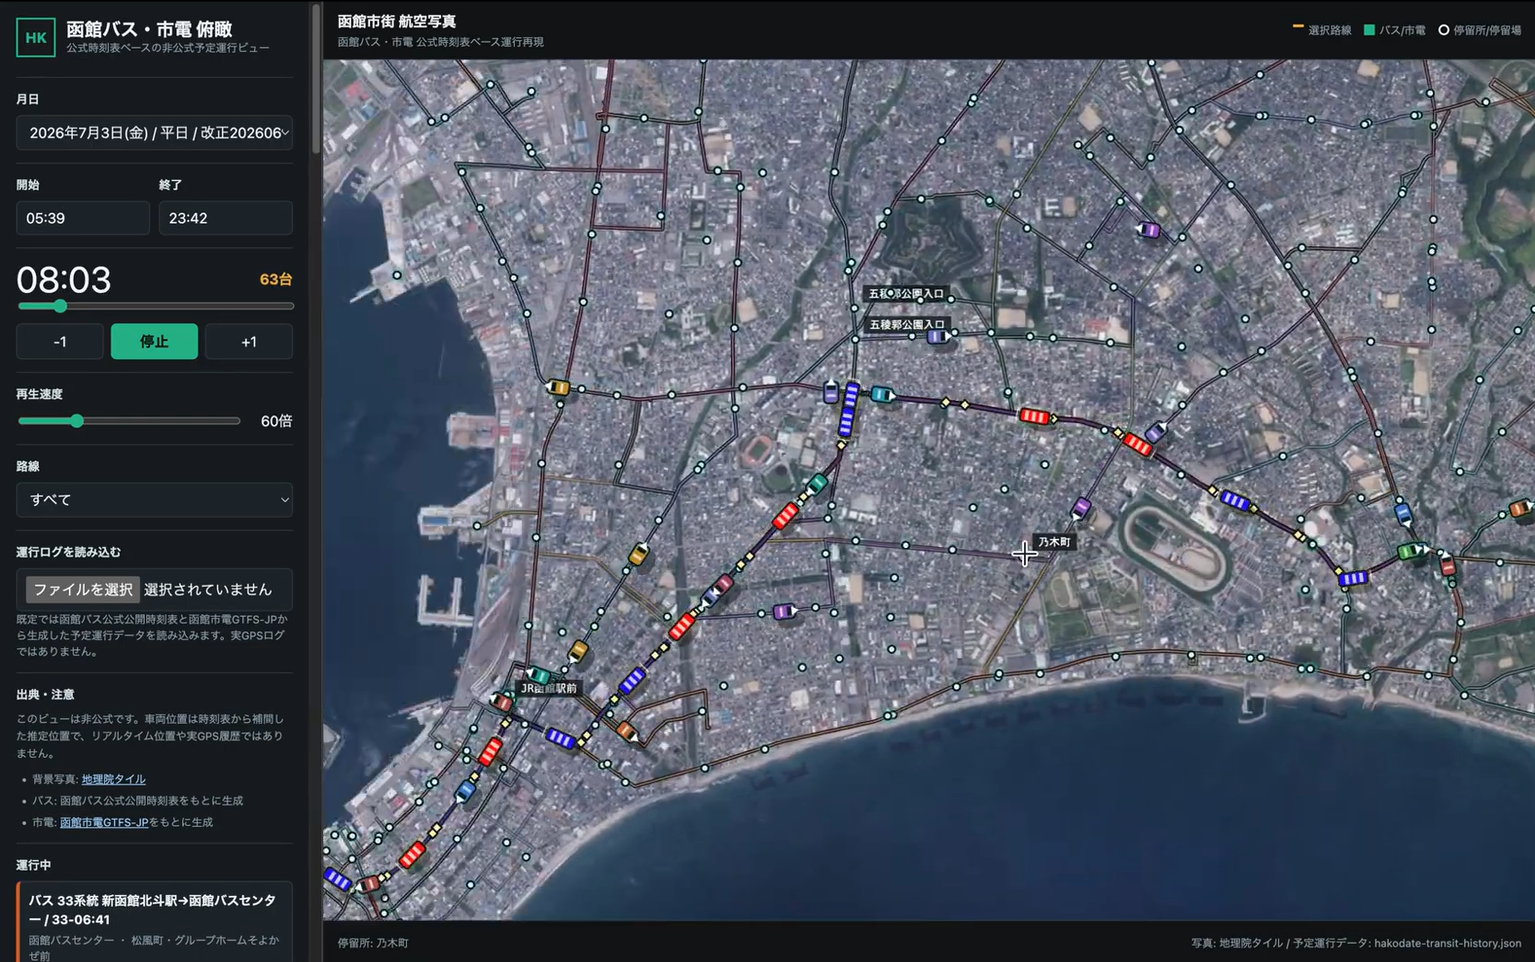
\includegraphics[width=0.95\linewidth]{figures/ch4_overview_sim.png}
  \caption{時刻表に基づく運行状況の可視化ツールの画面}
  \label{fig:overview-sim}
\end{figure}

調査の結果，計測を行った範囲では，登校時間帯に亀田支所前から未来大学方面へ乗車する利用者が多く，同停留所を出発した後に車内の乗客数が増加する傾向が確認された．また，授業開始時刻に間に合う一部の便に利用者が集中しており，混雑は路線全体に一様に発生するのではなく，亀田支所前からはこだて未来大学までの区間に集中していた．一方で，登校時間帯以外や対象区間以外では，同程度の利用者の集中は確認されなかった．

これらの分析により，特に登校時間帯の亀田支所前からはこだて未来大学までの区間に問題が集中していることを確認し，対策を検討すべき停留所や時間帯を絞り込んだ．
\bunseki{野澤遼大}

\subsection{解決策候補の比較検討}
本プロジェクトでは，未来大学行きのバスの混雑を緩和する方法について，グループで複数回の話し合いを行い，さまざまな解決策を検討した．

初めに，学生専用バスの運行，連節バスの導入，快速バスの導入など，複数の案を挙げ，それぞれのメリットやデメリットについて議論した．検討した主な案の比較を表~\ref{tab:solution-comparison} に示す．なお，検討初期には，通学全体の利便性を向上させる案として深夜バスも挙げたが，登校時間帯の混雑を直接緩和する案ではないため，主要な候補から除外した．学生専用バスは混雑を大きく緩和できる可能性がある一方で，新たな車両や運転手の確保が必要となるため，実現には多くの費用がかかると考えられた．また，連節バスについても輸送能力は高いが，車両の導入や道路環境などの課題があり，短期間で実施することは難しいと考えられた．

その中で，快速バスの導入は，新たな車両や運転手を必要とせず，既存の運行ダイヤを大きく変更せずに実施できることから，最も実現可能性の高い解決策であるという結論に至った．快速バスであれば，一部の停留所を通過することで所要時間を短縮でき，利用者を通常便と分散させることによって混雑の緩和が期待できる．

\begin{table}[H]
  \centering
  \caption{検討した解決策の比較}
  \label{tab:solution-comparison}
  \begin{tabular}{|l|p{22mm}|p{27mm}|p{28mm}|p{28mm}|}
    \hline
    項目 & 深夜バス & 学生専用バス & 快速バス & 連節バス \\
    \hline
    メリット &
    ・ニーズはある &
    ・授業時間に合わせて運行できる\par ・混雑緩和\par ・利用者層が明確 &
    ・時間短縮\par ・遅延しにくい\par ・混雑緩和 &
    ・多くの乗客が乗れる\par ・混雑緩和につながる \\
    \hline
    デメリット &
    ・運転手不足\par ・需要予測が難しい &
    ・運転手不足\par ・コストが高い &
    ・利用者が少ないと意味がない\par ・通過される停留所の利用者の利便性が低下する &
    ・専用車両導入のためコストや手間がかかる\par ・高い運転技術が必要 \\
    \hline
  \end{tabular}
\end{table}
\bunseki{野澤遼大}

\section{解決策の提案}
本プロジェクトでは，亀田支所前からはこだて未来大学まで運行している既存のバスの一部を快速バスとして運行することを提案する．快速バスは，利用者の少ない停留所を通過し，亀田支所前とはこだて未来大学を短時間で結ぶことを目的とする．一方で，通常便はこれまで通り全ての停留所に停車するため，途中停留所の利用者にも配慮した運行が可能である．

本プロジェクトで提案する快速バスは，単に移動時間を短縮することだけを目的としているわけではない．快速化によって一回の運行時間を短縮し，その短縮できた時間を利用して，同じ車両が混雑区間である亀田支所前からはこだて未来大学までの区間をもう一度運行することを想定している．つまり，新たにバスを増便するのではなく，既存の車両の運行方法を工夫することで，混雑区間の輸送力を向上させようという考え方である．快速バス運行案の概要を図~\ref{fig:rapid-bus} に示す．

\begin{figure}[H]
  \centering
  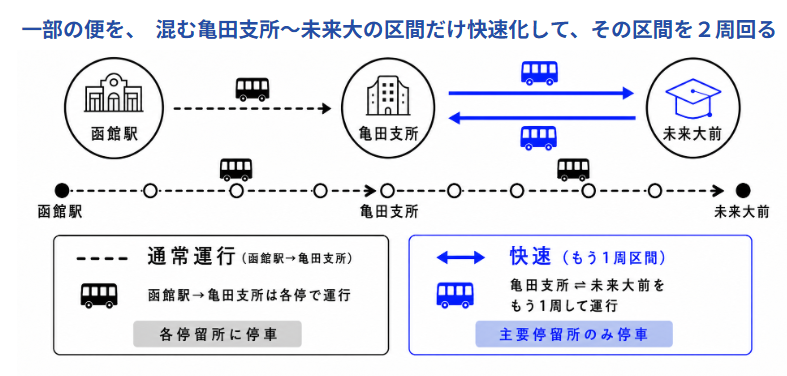
\includegraphics[width=0.9\linewidth]{figures/ch4_rapid_bus.png}
  \caption{快速バス運行案の概要}
  \label{fig:rapid-bus}
\end{figure}

これにより，未来大学へ向かう学生の一部を快速便に誘導し，通常便への利用者集中を分散できると考えた．その結果，混雑の緩和だけでなく，乗降時間の短縮や遅延の減少，利用者の移動時間の短縮などの効果が期待できる．また，新たなバスを増便するのではなく，現在運行している便の一部を快速化するため，大きな設備投資を必要とせず，比較的実現しやすい点も特徴である．

この解決策の特徴は，「バスを増やす」のではなく，「運行方法を最適化する」ことで混雑の緩和を目指している点にある．なお，快速バスの有効性は感覚的に判断するのではなく，数理モデルを用いたシミュレーションによって定量的に評価する．その具体的な計画については\chapref{plan}で述べる．
\bunseki{本光世奈}

\section{期待される効果と留意点}
\enlargethispage{3\baselineskip}%
快速バスを導入することによって，学生・バス事業者・地域の三者に対して様々なメリットが期待できる．学生にとっては，利用者が通常便と快速便に分散することで積み残しが減少する可能性がある．また，一部の停留所を通過することで所要時間が短縮され，通学時間の短縮や快適性の向上も期待できる．さらに，乗降にかかる時間が短くなれば，遅延の改善にも繋がる可能性がある．バス事業者にとっては，新たな車両を導入せずに既存の便を活用できるため，大きなコストをかけずにサービス改善を図ることができる．また，混雑が緩和されることで利用者満足度が向上し，公共交通の利用促進にもつながると考えられる．地域にとっても，公共交通が利用しやすくなれば，自家用車の利用抑制や交通渋滞の緩和など，間接的な効果が期待できる．

一方で，快速バスには留意すべき点もある．快速便が通過する停留所を利用する人にとっては，乗れる便が減り，待ち時間が長くなる可能性がある．また，快速便に利用者が集中しすぎると，通常便との混雑の差が大きくなり，期待したほど混雑が分散しない可能性もある．

そのため，快速バスの導入を考える際には，学生の利便性だけでなく，通過停留所の利用者への影響や，通常便と快速便のバランスを評価する必要がある．
\bunseki{本光世奈}

\include{chapter5}

%========= 参考文献 ===========
\begin{thebibliography}{9}
\bibitem{book1} R. S. Sutton and A. G. Barto, Reinforcement Learning, MIT Press, USA, 1998.
\bibitem{paper1} A. J. Smith and K. Taro, ``The applications of the self-organising map to reinforcement learning," Neural Networks archive, vol. 15, Issue 8-9 , pp. 1107--1124,  Oct. 2002.
\end{thebibliography}

%========= 付録 ===========
\begin{appendix}
\chapter{章のタイトル}
─内容─
\section{節のタイトル}
─内容─
\section{節のタイトル}
─内容─


\chapter{グループ報告書執筆要項}
\section{記載内容}
\noindent
●記載内容の一例を以下にまとめる\\
・表紙：プロジェクトの情報（フォーマット参照）\\
・日本語概要：目的，方法，結果，結論\\
・英語概要：同上\\
・キーワード\\
・背景\\
・プロジェクトで使用した従来技術\\
・制作物や活動内容の説明\\
・結果\\
・結論\\
・参考文献\\
・付録\\
\\
●章構成\\
・任意（担当教員の指示に従うこと）\\
\\
●フォーマット\\
・Texファイル（ｐｄｆファイル）に準じること．\\
・分量：制限なし\\
\\
\section{報告書に関する手続き}
\noindent
●報告書の確認\\
・プロジェクト担当教員に確認してもらうこと．\\
\\
●報告書作成ツール\\
○本文\\
・プロジェクト担当教員の指示に従うこと．\\
○図表など\\
・プロジェクト担当教員の指示に従うこと．\\
\\
%●提出方法\\
%・ファイル形式：ｐｄｆ\\
%・提出場所：プロジェクト学習WGの指示に従うこと．\\
%・ファイル名groupXXY.pdf\\
%　XX：プロジェクト番号（２桁：01,02,03…）\\
%　Y：グループ番号（大文字アルファベット：A,B,C,…，1グループの場合は、Aとすること.）\\
%  例：プロジェクト２，グループＢの場合：group02B.pdf\\

\end{appendix}

\end{document}
